\documentclass[letterpaper,twocolumn,10pt]{article}
\usepackage{final-resources/usenix,epsfig,endnotes,enumerate,graphicx}
\begin{document}

%don't want date printed
\date{}

%make title bold and 14 pt font (Latex default is non-bold, 16 pt)
\title{\Large \bf Distributed Ray Tracing: Parallelizing graphical computation\\
  \small \normalfont by \#ConcurrentSwag}

\newcommand{\tuftsauthor}[1]{{\rm #1}\\
  Tufts University}

\author{
  \tuftsauthor{Arthur Berman}
  \and
  \tuftsauthor{Maxwell Bernstein}
  \and
  \tuftsauthor{Thomas Colgrove}
  \and
  \tuftsauthor{Kate Wasynczuk}
}

\maketitle

% Use the following at camera-ready time to suppress page numbers.
% Comment it out when you first submit the paper for review.
%% \thispagestyle{empty}


\subsection*{Abstract}
We want to parallelize ray tracing across multiple machines instead of just
multiple processes on one machine. These machines and processes need to
communicate.

\section{Design}

We have a not-so-thin-server (``Collector''), and heavy-client (``Worker'')
approach, where the Collector controls the scene(s) being worked on, and sends
them to Workers to be rendered.

We chose this design because it offers the most extensibility and least amount
of mutable resource sharing. It is also the easiest to employ in a practical
manner. We could from this state create a wrapper for both Collectors and
Workers, called Manager. This manager could orchestrate multi-scene rendering
efforts, spin up remote workers, and more.\\ %% need line break here

\begin{center}
  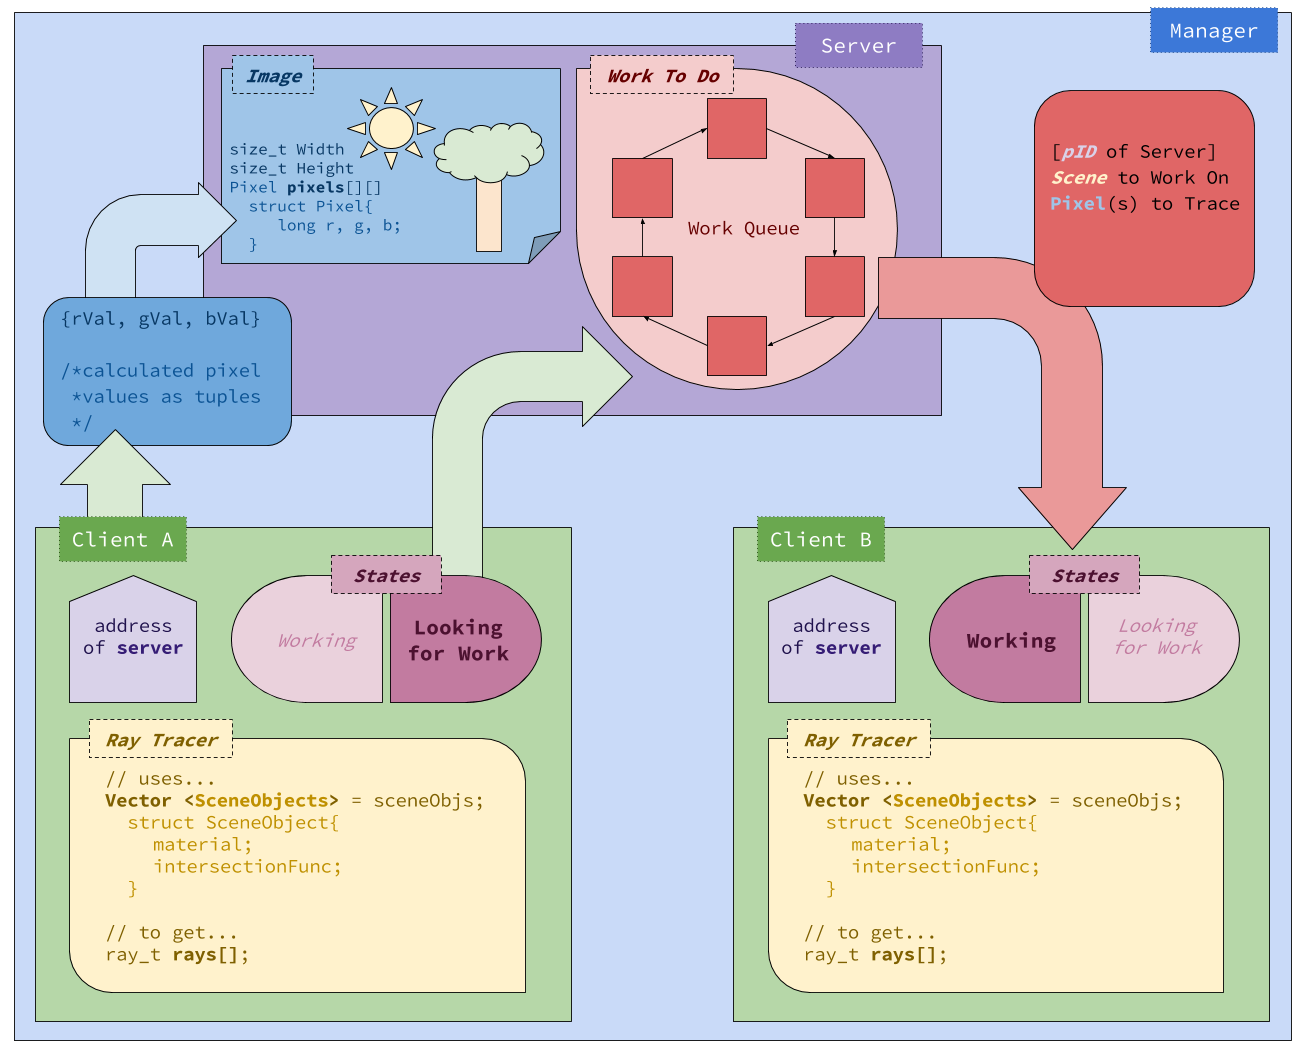
\includegraphics[height=60mm]{obj-diagram.png}
\end{center}

In this state, we see two Workers and one Collector. The Collector is attempting
to render an image with an arbitrary width and height. The Collector can be in
one of two states: assigning work, and outputting image. When the Collector is
assigning work, it waits for messages from Workers, then allocates work to each
Worker that asks. The Collector selects work based on the current front of a
circular queue. Once work is complete (read: returned by a Worker), it is
removed from the queue.

Work consists of a named scene description file and a set of pixels. Once every
pixel in the image has been rendered, the Collector transitions to outputtting
an image.

When the Collector is outputting an image, the Collector writes a file to the
filesystem containing the rendered image.

There are two Workers connected to the server. Worker A is looking for work.
Worker B has received work and is working. Worker A has sent a message to the
server requesting a set of pixels. When the server responds, Worker A will
transition to the working state.

Worker B, in the working state, is iterating through the set of pixels in its
packet of work. For each pixel, it uses a traced ray to determine the correct
color. Once all pixels have been rendered, it returns the set of rendered colors
to the server and transitions to the look for work state.

\section{Reflection on design}

The two best design decisions we made work hand in hand: the work queue, and the
stateless message protocol.

The work queue allows for clients to fail for whatever reason (network issues,
segfaults, etc) and the image to continue to be rendered successfully.

The stateless message protocol accomplishes the following:

\begin{itemize}
\item Limit number of open connections.
\item Reduce complexity in both Worker and Collector state machines.
\item Limit technology requirements (i.e. no keep-alive connections,
  long-polling, etc)
\end{itemize}

%% \section{Completed work}

%% \begin{enumerate}[(a)]
%% \item Developed a clear client/server architecture.

%% \item Extensively researched ray-tracing algorithms.

%% \item C++ classes for core data structures and modules (PNM
%%   rendering, vector math, objects in 3D space, pixels, etc).

%% \item TCP client and server implementations.

%% \item Request-response protocol using said TCP client and server.

%% \item Work-pooling algorithm that distributes work in an optimal and
%%   deterministic fashion.

%% \item Completed distributed ray tracer.
%% \end{enumerate}

\section{Analysis of outcome}

We were able to achieve our minimum and maximum deliverables from the initial
proposal and further. We can, by means of a Python script, also create moving
GIFs of renders of scenes. See the example of snowman with snow falling.

The math, while difficult, did not prove nearly as intractable as we initially
thought, \textit{even though} we do not have backgrounds in mathematics.
Additionally, the math required for ray tracing allows for easy frame
splitting. We were not sure if this was possible.

\section{Reflection on development plan}

We operated in two-week sprints as pairs. Each pair followed the COMP 40
pair-programming paradigm, with two members of the group on one computer, with
one driving and the other providing continual feedback.

At the end of each sprint, each pair pushed the code to a feature branch, and
then pair reviewed the other pair's code. After pair review (and appropriate
revisions), feature branches were merged into the development branch.

\subsection{Sprints}

\begin{enumerate}[(1)]
\item Thomas and Max: single-threaded ray tracer, Kate and Arthur: scene
  description parser

\item Thomas and Arthur: integrate ray tracer and scene description parser, Kate
  and Max: networking stack, message passing, and work queue

\item Arthur and Max: integrate work queue and message passing into ray tracer,
  Thomas and Kate: slide deck and presentation materials
\end{enumerate}

\subsection{Reflection}

For the most part, the pair-sprint format worked well. It forced every member of
the group to have a solid understanding of the code and the architecture.
Additionally, it ensured punctuality by way of peer pressure.

Occasionally, one team would require assistance from another in order to finish
a sprint.

\subsection{Interface management}

The weekly full-group meetings to decide interfaces worked well. We found that
in practice, a team would make the call to change an interface in order to write
better code. This was not a problem.

\section{Bug report}

We had several difficult bugs, one of which we have still not managed to track
down.

\subsection{JSON? What JSON?}

Occasionally, the Worker would have trouble parsing larger scene files sent by
the Collector. JsonCpp would complain about poorly formed documents, that it
expected an open brace here, quote there, etc. Even after very detailed manual
inspections, the transmitted JSON appeared completely fine.

One time, however, Max noticed a non-ASCII character rendered as a question mark
in the JSON output. This kind of output only appears when the terminal can't
render the (presumably invalid) character. On larger JSON files, these question
mark characters appeared at very regular intervals - about every 512 bytes, the
amount we \verb|recv()| each call.

It turned out that the amount we \verb|recv()|'d completely filled our buffer,
leaving room for no NUL-terminator, so we would read past the bounds of buffer
whenever we loaded JSON. If we \verb|recv()|'d one less character, the problem
disappeared.

\subsection{SIGBUS...?}

After debugging the JSON issue mentioned above, the Worker could parse JSON,
render pixels, and then send to the Collector. However, the Collector would exit
with SIGBUS on images larger than roughly 200 by 300 pixels. When Max ran the
Collector under gdb and unrolled the stack, there were nearly 500 stack frames
of the same function - \verb|read_from_sock|.

\verb|Read_from_sock|, given a client socket and string buffer reference, will
read until there is nothing more to read, and append the buffer to the string
all the while. It was initially written recursively because it was the cleanest
way - however, it looked like on large messages (which could be up to five (5)
megabytes) and chunk sizes of 512 bytes, there would be a stack overflow that
only got noticed when \verb|read_from_sock| tried to \verb|bzero()| a variable.

\verb|Read_from_sock| was rewritten as an iterative function, and order was
restored.

\subsection{JsonCpp keeps global state}

We use JsonCpp as our JSON serialization and deserialization library. This is
for the most part an excellent library, but when we started running into errors
when ray tracing with multiple Workers. We noticed that JsonCpp would
occasionally throw a runtime error about blowing the stack. This error message
only cropped up when using two or more Workers.

Max decided to track down where this error message came from, and found out that
there was an artificial cap on the recursion allowed in the JSON parser.
Interestingly enough, the recursion count was kept in a \textit{global
  variable}, allowing all instances of the \verb|Json::Reader| class to
increment it at the creation of each new stack frame. Naturally, we ``blew the
stack'' early and often.

The fix (submitted as a pull request to the JsonCpp project) is to localize the
\verb|stackDepth| variable to each instance of the \verb|Json::Reader| class by
making it a member variable. The problem disappears after patching the library.

The team submitted a pull request to the JsonCpp library with a fix for the
issue.

\subsection{Sockets randomly closing}

Currently, Workers will fail to \verb|send()| messages, exiting the process with
an error about using the wrong protocol for that type of socket. After some
preliminary internet research, this error can occasionally appear when trying to
\verb|send()| large messages. Our messages can be very large, so Max wrote some
code to split the larger messages into 512 byte chunks and \verb|send()| those
instead.

Instead of fixing the problem, the Workers then exited with SIGPIPE. At some
point during the repeated \verb|send()|s, the pipe was closing and Workers could
no longer write.

While researching the SIGPIPE errors after the presentation, Max realized that a
SIGPIPE indicates that the connection is no longer open, and the socket is
invalid. Perhaps it was not some bizarre system issue after all! After some
investigation into the `TCPServer' class, it became evident that the unforgiving
timeout in \verb|read_from_sock| closed the connection too early. The timeout
was increased from 0.01 seconds to 1 second and all was well.

\section{Code overview}

%% TODO: put stuff here

\section{Update from final design}

In this section, we update the grading reader on the project's progress since
the last submitted document. Sections that have not changed are omitted, and
some new sections are added.

\subsection{Progress}

We can fully render spheres with diffuse color, reflection, and refraction. We
are able to render a single image across multiple processes and multiple hosts.

%% TODO: add more


\section{Update from initial design}

\subsection{Diagrams}

We have updated the vocabulary in the diagram obj-diagram.png to reflect 
an accurate description of the roles of various processes in the system.

\subsection{Progress}

We can adequately render spheres with diffuse color, and load a scene from
an external description. We are able to render frames in independent processes,
but cannot yet render a single image across multiple processes. 

\subsection{Vocabulary}

We have transitioned from the terms ``Client'' and ``Server'' to the terms
``Worker'' and ``Collector.'' Worker processes handle rendering of an arbitrary
chunk of the image, which it then sends to the collector process, which collects
rendered chunks and assembles them into a finished image.


\end{document}
